%% This is the first chapter.  
%% You should put chapter/appendix that you write into a separate 
%% file, and add a line \include{yourfilename} to main.tex
\chapter{Introducción} \label{Intro} 
\chaptermark{Introducción} \lettergroup{\thechapter}

Este texto es simplemente para poner un ejemplo de cita \cite{Yandell2012} y otro de glosario como \gls{foobar} o \gls{SVM}

\section{Motivations}
\lipsum[1-4]

\section{Description}

%% Box
\begin{tcolorbox}[colback=blue!5,colframe=blue!40!black,title=Box 1: ]
\lipsum[2]
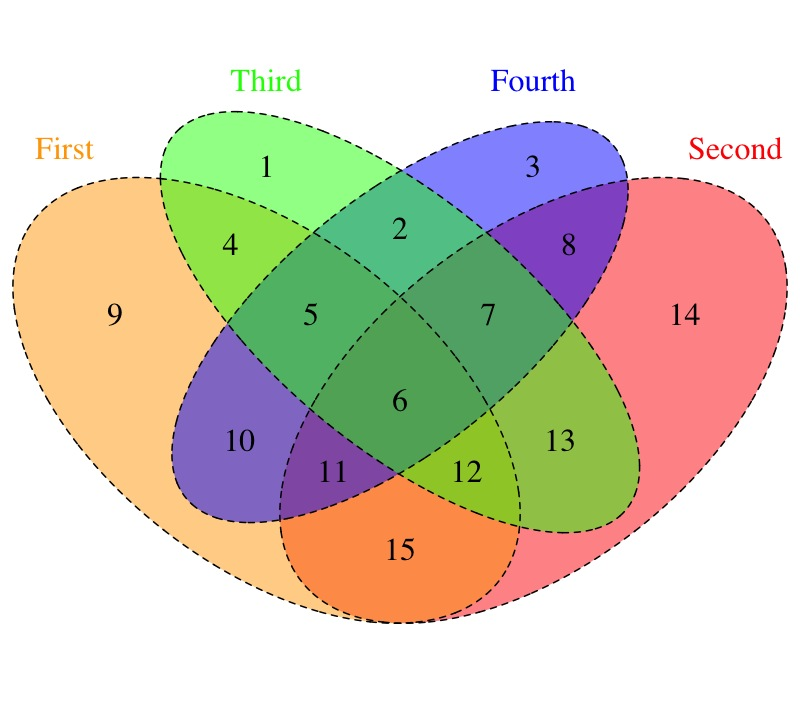
\includegraphics[scale=0.15]{figures/Venn}
\end{tcolorbox}

\subsection{Post}
\lipsum[1-2]

\begin{figure}
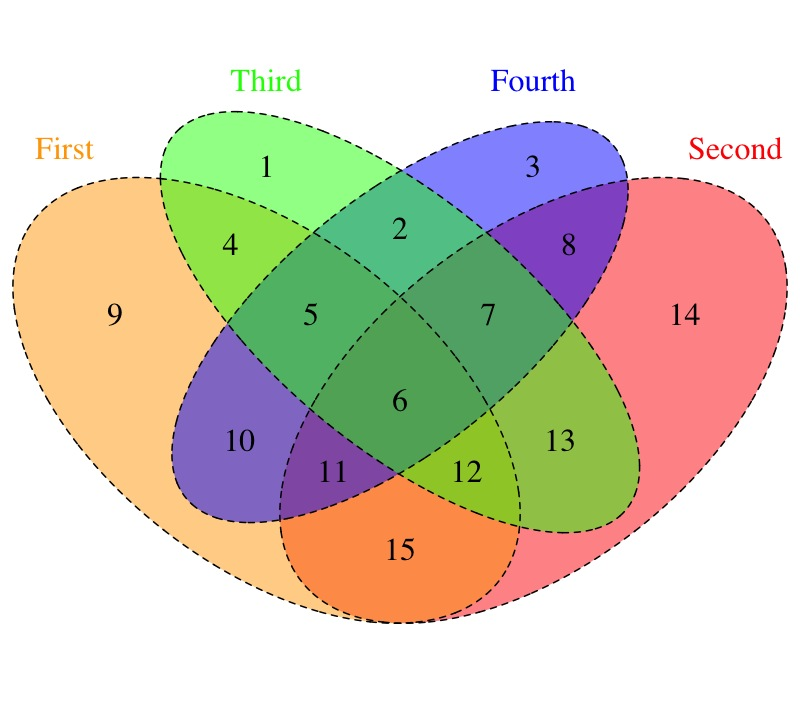
\includegraphics[scale=0.15]{figures/Venn}
\caption{example test text}
\label{fig:Venn}
\end{figure}

\lipsum[1]

\section{Sección}
texto

\subsection{Subsección}

texto



